% I have provided the source and required media for this presentation
% under the hope that it will be useful. Please don't use it for
% anything nefarious.

% Also, note that this LaTeX file requires the beamer class to
% compile. If you don't already have it, you are expected to obtain
% and install it from http://latex-beamer.sourceforge.net/

% (c) 2011 -- Harish Narayanan

\documentclass[ignorenonframetext]{beamer}

\usepackage{graphicx}
\usepackage{amsfonts}
\usepackage{amssymb}
\usepackage{fancyvrb}
\usepackage{color}
\usepackage{multimedia}
\usepackage[english]{babel}
\usepackage[latin1]{inputenc}
\usepackage{textcomp}

% Custom commands

\newcommand{\references}[1] {
  \begin{flushright}
    \scriptsize [#1] \normalsize
  \end{flushright}
}

\newcommand{\addfigure} {
  \scriptsize
  \textcolor{red}{[insert figure]}
  \normalsize
}

% All sorts of things pertinent to styling beamer
\usetheme{boxes}
\setbeamertemplate{navigation symbols}{}
\usecolortheme{seagull}
\usefonttheme{professionalfonts}
\useinnertheme{circles}
\setbeamercolor{frametitle}{fg=red}
\setbeamercolor{title}{fg=red}

\mode<presentation> {
  \setbeamercovered{transparent}
}

\title{Electrophysiological modelling of chondrocytes in human
  articular cartilage}
\author{H.~Narayanan}
\subject{}
\institute[]{}
\date[]{}

\begin{document}

% 0. Title slide and mapping
%
%   Electrophysiological modelling of chondrocytes in human articular
%   cartilage
%
%   - Introducing the chondrocyte and why it is interesting in the
%     context of cartilage
%   - Some particular scientific questions
%
%   - Model and motivation
%   - Preliminary results
%   - Discussion

%\frame{\titlepage}

% Mapping slide containing visual outline
\begin{frame}
  \frametitle{This talk will Electrophysiological modelling of
    chondrocytes in human articular cartilage}
  \begin{columns}
    \begin{column}{3cm}
      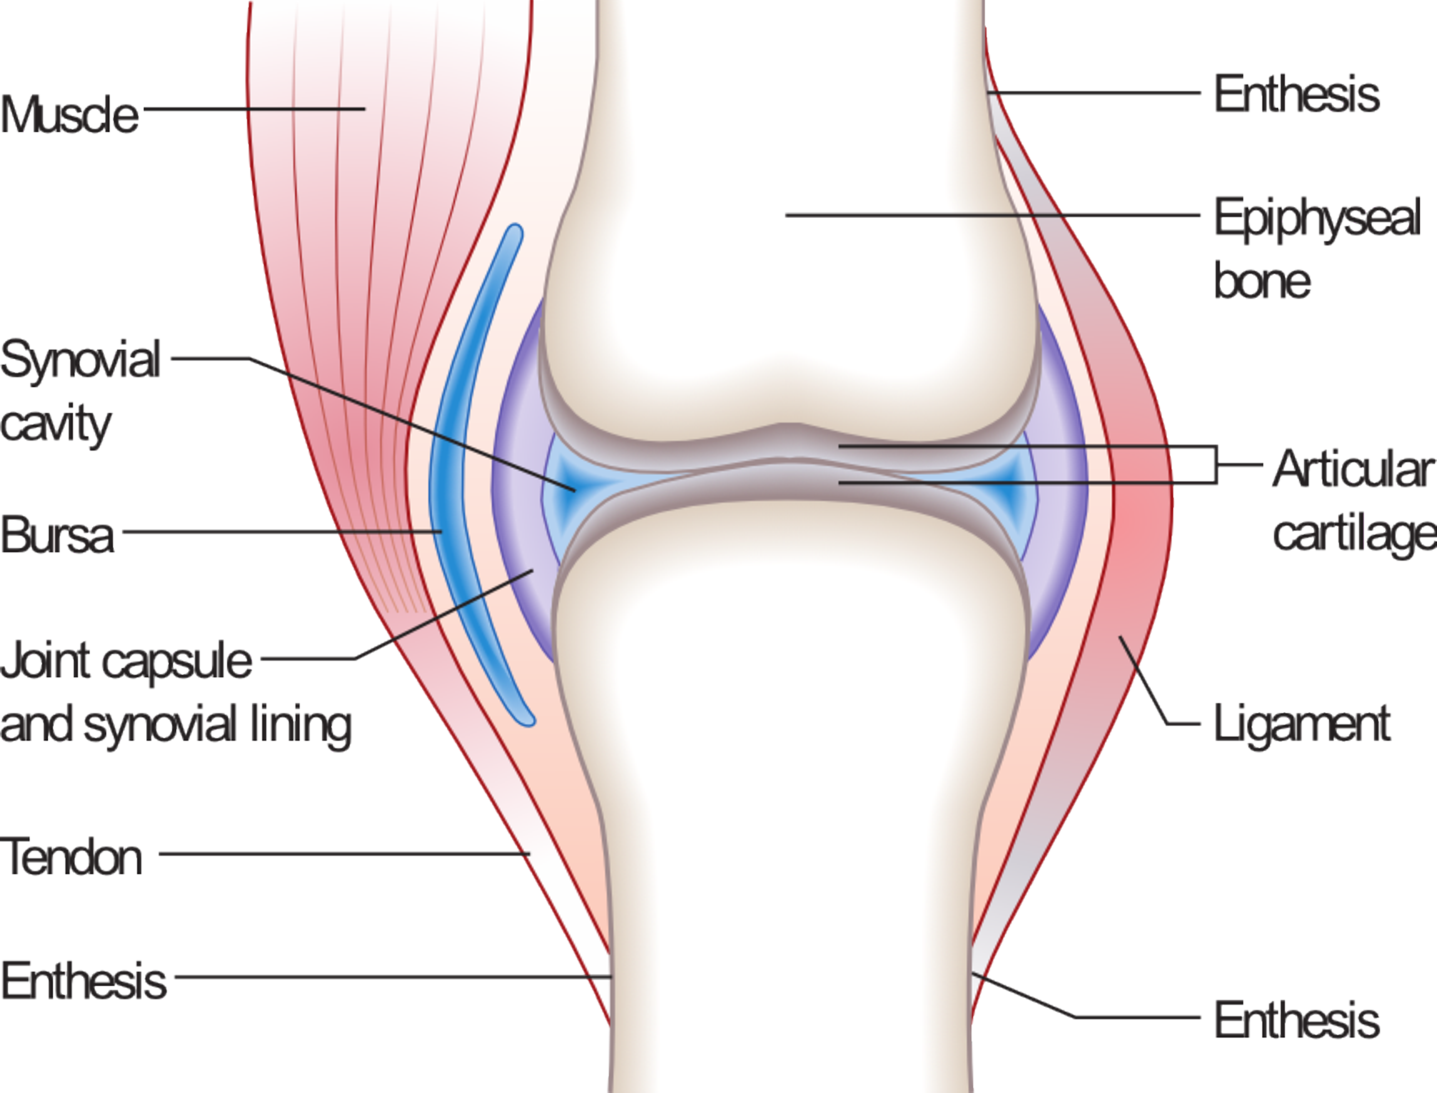
\includegraphics[width=2.5cm]{../images/pdf/joint}
    \end{column}
    \begin{column}{9cm}
      What is the chondrocyte and why is it interesting?
    \end{column}
  \end{columns}
  \vspace{0.2cm}
  \begin{columns}
    \begin{column}{0.5cm}
      % Empty
    \end{column}
    \begin{column}{4.5cm}
      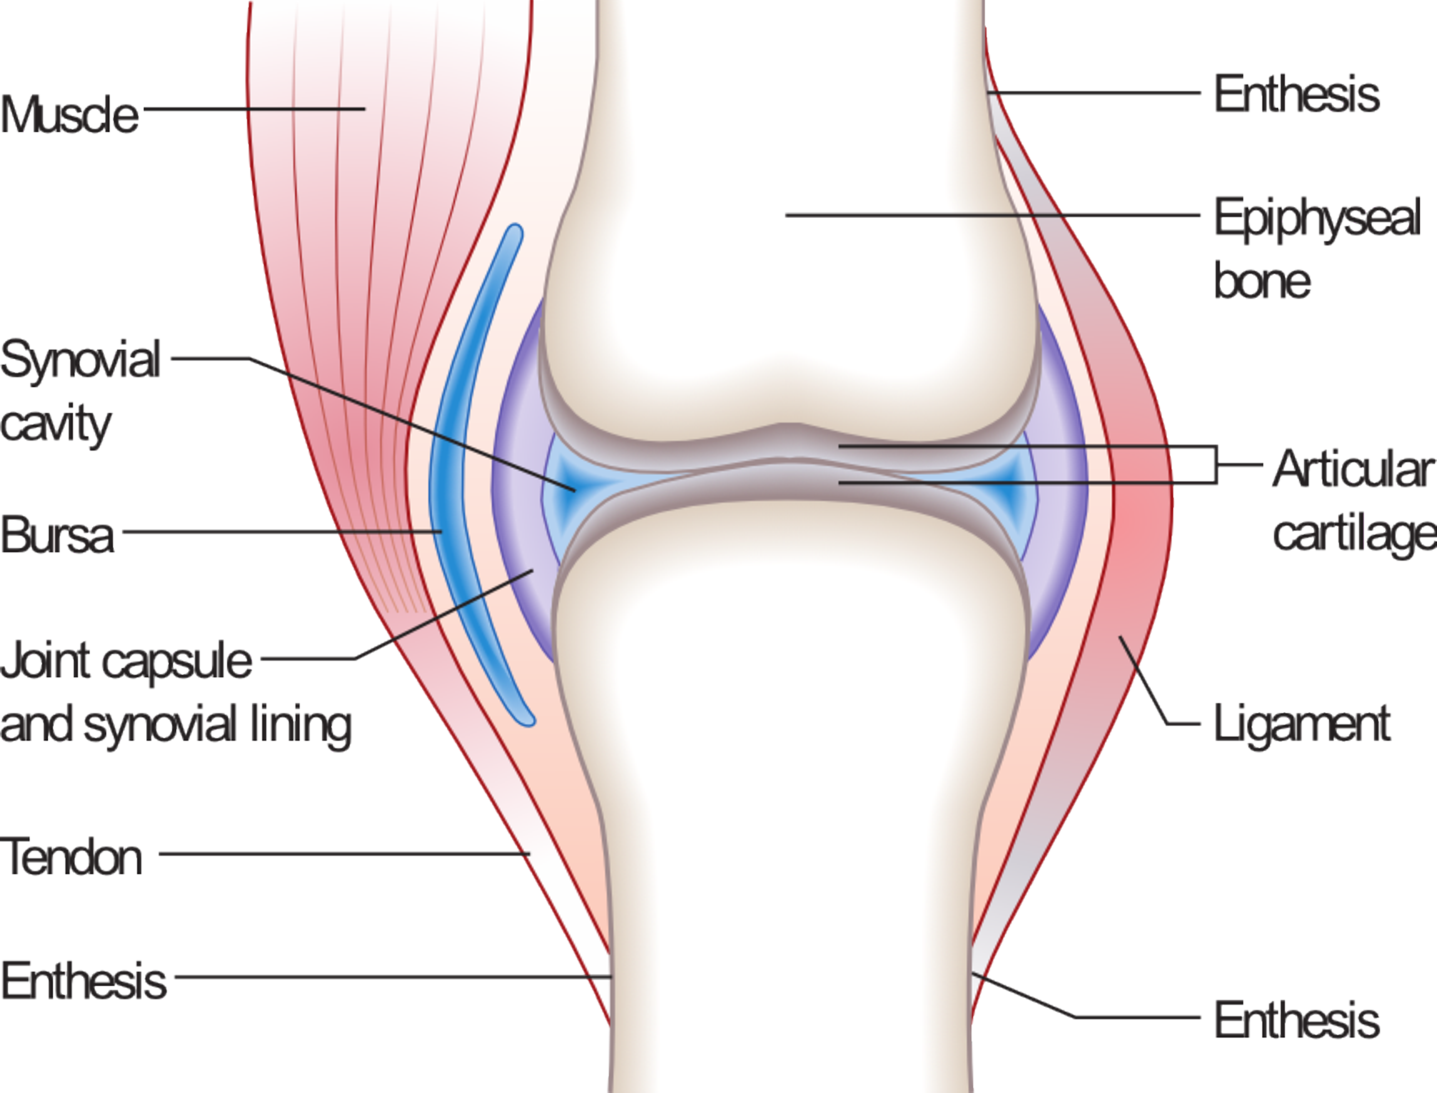
\includegraphics[width=2.5cm]{../images/pdf/joint}
    \end{column}
    \begin{column}{7cm}
      What are the specific questions we aim to answer?
    \end{column}
  \end{columns}
  \vspace{0.2cm}
  \begin{columns}
    \begin{column}{3.5cm}
      % Empty
    \end{column}
    \begin{column}{3cm}
      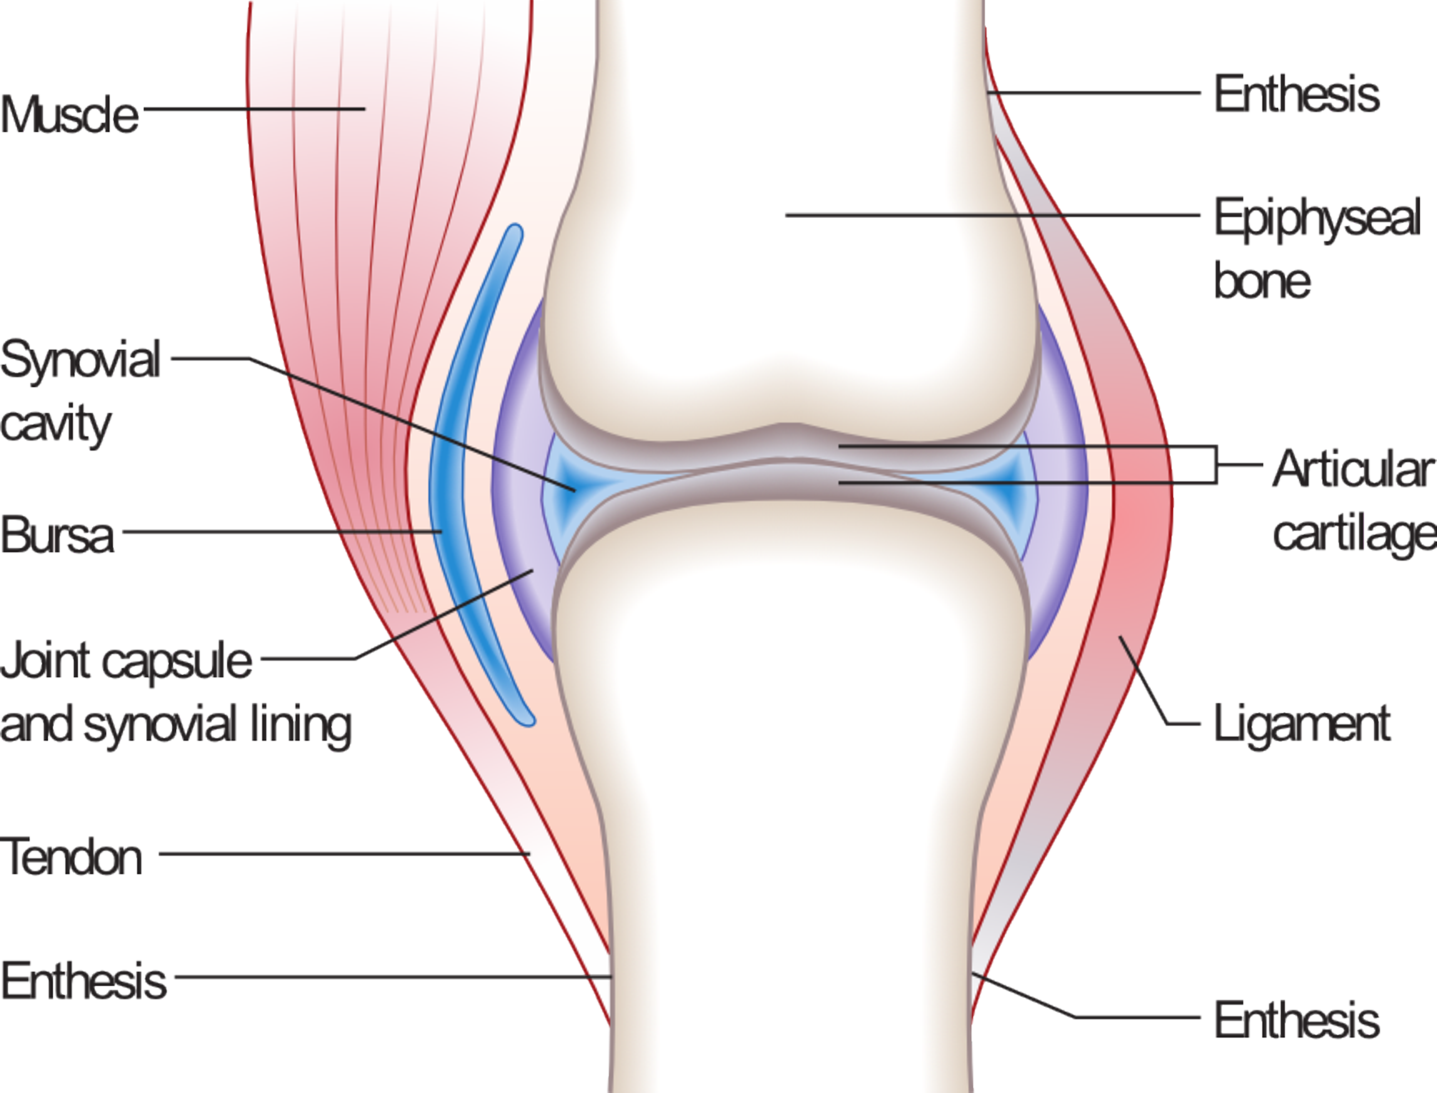
\includegraphics[width=2.5cm]{../images/pdf/joint}
    \end{column}
    \begin{column}{0.5cm}
      % Empty
    \end{column}
    \begin{column}{5cm}
      How we about modelling to do so?

    \end{column}
  \end{columns}
\end{frame}

% 1. What is the chondrocyte and why is it interesting?

\begin{frame}{Articular cartilage is the connective tissue that
    separates bones at joints, allowing them to slide past each other}

  \begin{columns}

    \begin{column}{6cm}
      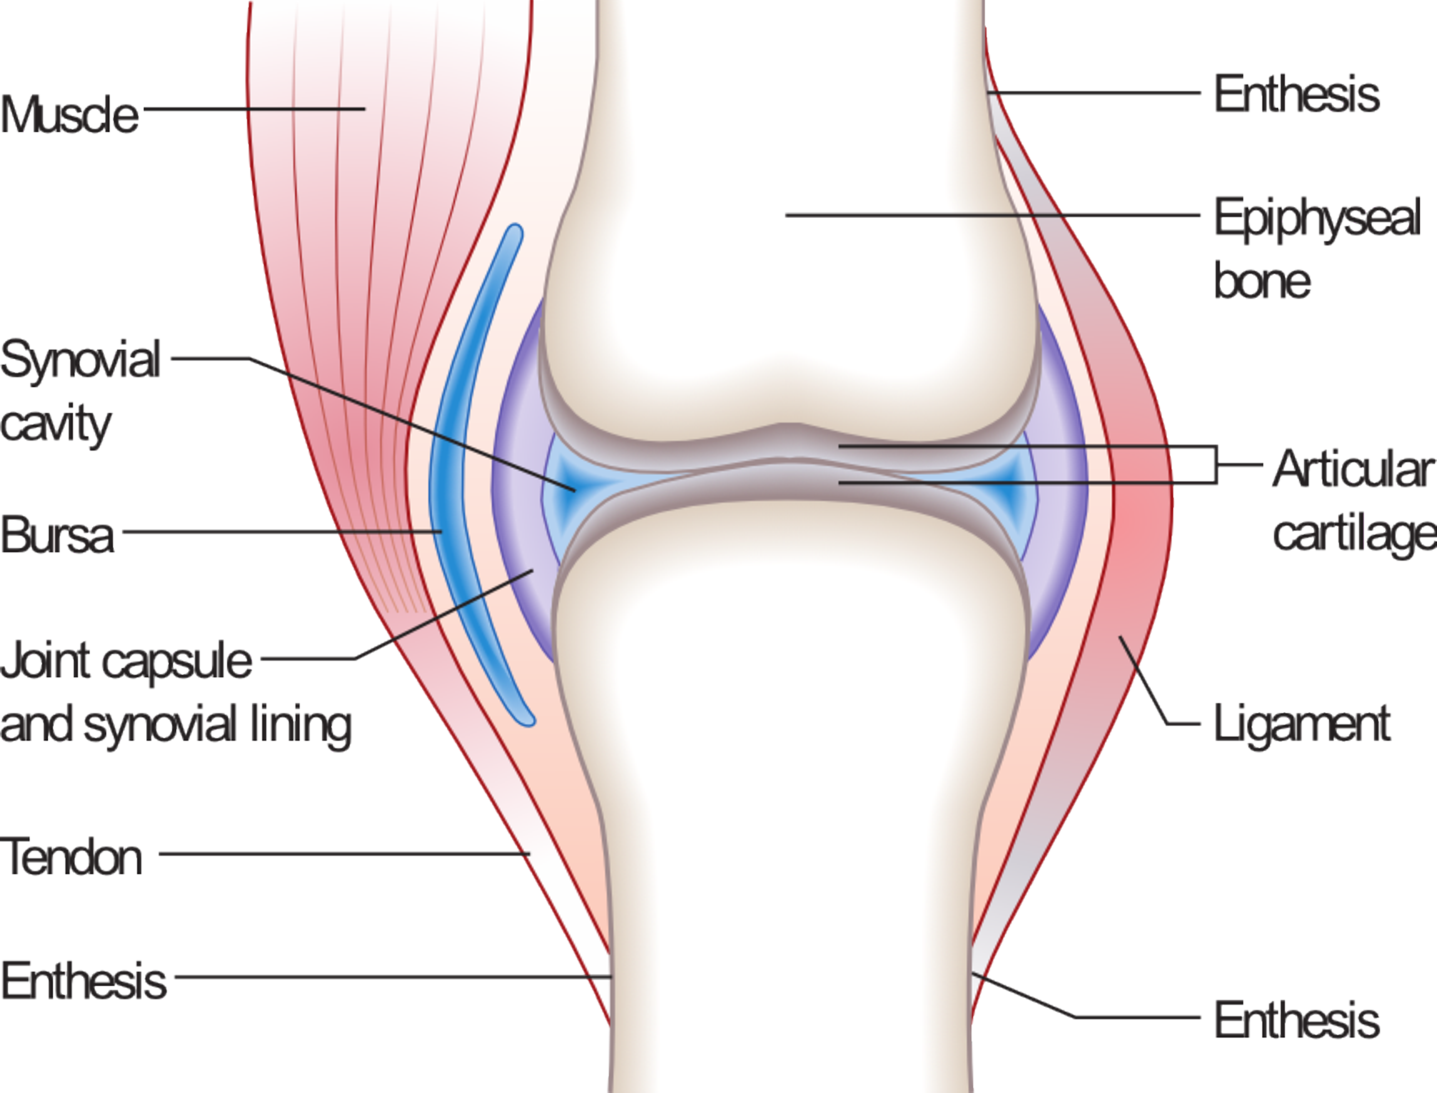
\includegraphics[width=6cm]{../images/pdf/joint}
    \end{column}

    \begin{column}{6cm}
      \begin{itemize}
      \item<1-> Cartilage is composed of chondrocytes, an ECM (collagen
        and elastin) and proteoglycans\\[0.5cm]
        \pause
      \item<2-> Cartilage is aneural, avascular and alymphatic and is thus
        slow to grow and heal % and relatively easy to study mathematically?
      \end{itemize}
    \end{column}

  \end{columns}

\end{frame}

\begin{frame}{Chondrocytes are the resident cells of articular
    cartilage and are responsible for maintaining the extracellular
    matrix}

  \begin{itemize}
  \item Low cell to tissue volume ratio (few \%), but can do a lot
  \item Signalling (pH sensitivity, ionic content, mechano-sensing
    (stress))---causes matrix synthesis/degradation
  \item Something in general about disruption?
  \end{itemize}

  \references{Poole, 1997; Archer \& Francis-West 2002}

\end{frame}

% A lot can happen, but we are interested in something particular
%
% 2. The specific question(s) we want to answer

\begin{frame}{We narrow our focus to specific questions to motivate
    our initial modelling efforts}

  \begin{itemize}
  \item Hypothesis 1: ``Frozen shoulder syndrome'' when tissue is
    exposed to buvipicane (and its links to $I_{K_{2-pore}}$)
  \item Hypothesis 2: pH and volume regulation (via ASIC)
  \item Hypothesis 3: Apoptosis and osteoarthritis?
  \end{itemize}

\references{citation 1; Lewis et al., 2011; citation 3}

\end{frame}

% All of these need a good understanding of important channels
% => basis of resting membrane potential => volume regulation etc.
%
% There is a dearth of good biophysical models for this cell type and
% so we construct our own.
%
% Return to review papers. As of 1996, it looked like [figure], and as
% of 2011 people feel it looks like [figure], so on the whiteboard in
% my office you have a superset of these studies.
%
% 3. Modelling the electrophysiology of a single cell

\begin{frame}{What physiology literature tells us about the channels\\
    in chondrocytes}

  \begin{itemize}
  \item A superset of what is known thus far about the channels in the
    chondrocyte \addfigure
  \item Talk about some important ones and what their roles might be

    \references{Hall et al., 1996; Barrett-Jolley et al., 2010}

  \end{itemize}

\end{frame}

% And so, this is the model that is being researched and
% implemented. Removing the things that are not pertinent to humans
% etc., we end up with the following initial model.
%
% 4. The computational model

\begin{frame}{The electrophysiological model of a single cell}

  \begin{itemize}
  \item All channels we have decided to consider \addfigure %CellML
  \item Return to one specific hypothesis and point out the channels
    that seem important % Modify figure?
  \item Discuss some functional forms, including rationale
  \item Talk about the programming ideas
    \begin{itemize}
      \item ODE Solver
      \item Code layout
      \item Parameter estimation; genetic algorithm idea?
    \end{itemize}
  \end{itemize}

  \references{functional forms, Clark et. al, parameter estimation}

\end{frame}

% And with these parameters, I observe the following behaviour in my
% test cases
%
% 5. Some numerical simulations and their implications

\begin{frame}{What do the numerical simulations tell us?}

  \includegraphics[width=0.8\textwidth]{../results/pdf/membrane_behaviour}

  \begin{itemize}
  \item Attempts at determining parameters; tie with experimental data
  \item Basic benchmarking of the model; Testing our hypothesis?
  \end{itemize}

  \references{parameter estimation, benchmarking, hypothesis}

\end{frame}

% 6. Discussion

\begin{frame}{In conclusion, \ldots}

  \begin{itemize}
  \item Summarise what has been done
    \begin{itemize}
      \item Learnt a bit about the physiology of the chondrocyte
      \item Some ideas of the channels involved
      \item Arrived at some interesting questions
      \item A basic model to answer these questions
    \end{itemize}
  \item For the future
    \begin{itemize}
    \item Ask for modelling advice
    \item Implications of the calculations
    \item Tissue level models and stress response
    \end{itemize}
  \end{itemize}

  \references{code, paper}

\end{frame}

\end{document}

% Local Variables:
% mode: latex
% mode: flyspell
% mode: auto-fill
% End: